% !TeX spellcheck = de_DE
\documentclass[ngerman]{scrartcl} 

\KOMAoptions{fontsize=12pt, paper=a4}
\KOMAoptions{DIV=11}
\usepackage[utf8]{inputenc}             % Direkte Eingabe von ä usw.
\usepackage[T1]{fontenc}               	% Font Kodierung für die Ausgabe
\usepackage{babel}                   	% Verschiedenste sprach-spezifische Extras
\usepackage{parskip}
\usepackage[autostyle=true]{csquotes}	% Intelligente Anführungszeichen
\usepackage{amsmath}					% Mathematischer Formelsatz mit zusätzlichen mathematischen Schriften und Symbolen
\usepackage{amssymb}					% Mathematischer Formelsatz mit zusätzlichen mathematischen Schriften und Symbolen
\usepackage{physics}					% Differentialgleichungen
\usepackage{listings}					% Zum Einbinden von Programmcode verwenden wir das listings-Paket
\usepackage[dvipsnames]{xcolor}			% um Elemente von Befehlen farblich zu unterstützen
\usepackage[varg]{txfonts}              % Schönere Schriftart
\usepackage{graphicx}					% Paket um externe Graphiken einzufügen
\usepackage{media9}
\RequirePackage[backend=biber, style=numeric]{biblatex} % Literaturverzeichnis
\usepackage{hyperref} 					% um klickbare Elemente in Ihrem PDF-Ausgabedokument zu erzeugen
\RequirePackage[all]{hypcap} 			% ergänzend zu hyperref
\usepackage{siunitx}					% Intelligentes Setzten von Zahlen und Einheiten
\usepackage{enumitem}					% Aufzählungsarten
\usepackage{fancyhdr}


\setlength\parindent{0pt} 				% Sets paragraph indentation to 0

\lstset{									% Deutsche Umlaute
	basicstyle=\ttfamily,    
	literate={~} {$\sim$}{1} 				% set tilde as a literal
	{ö}{{\"o}}1
	{ä}{{\"a}}1
	{ü}{{\"u}}1
	{ß}{{\ss}}1
	{Ö}{{\"O}}1
	{Ä}{{\"A}}1
	{Ü}{{\"U}}1
}

\lstset{
	numbers=left, 						% Line numbering
	numberstyle=\footnotesize, 			% Size of numbers
	basicstyle=\ttfamily\small, 		% Style and Size of Text
	backgroundcolor=\color{White}, 		% Background Color
	language=Python, 					% Language of Code
	commentstyle=\color{Maroon}, 		% Color and Style of Comments
	stringstyle=\color{OliveGreen}, 	% Color of Strings
	showstringspaces=false,
	morekeywords={import,from,class,def,for,while,if,is,in,elif,else,not,and,or,print,break,continue,return,True,False,None,access,as,del,except,exec,finally,global,import,lambda,pass,print,raise,try,assert}, 									% Definition of new keywords that will be highlighted
	keywordstyle=\color{RoyalBlue}		% Color and Style of Keywords
}


\pagestyle{fancy}
\fancyhf{}
\rhead{Ben Karcher, Anika Hoverath}
\lhead{Computerphysik - Abgabe 5}
\rfoot{Seite \thepage}

\title{Computerphysik - Abgabe 5}
\date{\today}


\begin{document}
	% Auf 3 setzen, da es beim ersten Chapter um 1 hochgezählt wird. 3+1=42
	\setcounter{section}{9}
	\thispagestyle{fancy}
	\renewcommand{\thesection}{H.\arabic{section}:}
	\renewcommand{\thesubsection}{H\arabic{section}.\arabic{subsection}}
	
\section{Solitonlösungen der \textsc{Korteweg-de Vries}-Gleichung}

\textit{In diesem pdf-Dokument sind Videos eingebunden, diese werden leider nicht mit jedem pdf-Viewer korrekt angezeigt. Bitte verwenden Sie einen Viewer, der Videos unterstützt, wie zum Beispiel \emph{okular}. Sollte Ihnen dies nicht möglich sein, haben wir die .mp4-Dateien auch nochmal separat angefügt.}

In dieser Aufgabe untersuchen wir L\"ossungen der Korteweg-de Vries-Gleichung.
Diese gelichung beschreibt die Ausbreitung von Wellen in Kan\"alen.

\begin{equation*}
\frac{\partial}{\partial t} u(t, x)=6 u(t, x) \frac{\partial}{\partial x} u(t, x)-\frac{\partial^{3}}{\partial x^{3}} u(t, x)
\end{equation*}

Eine besonderer Satz L\"ossung sind die Solitonen.
Diese beschreiben einzelne Wellen die sich mit konstanter geschwindigkeit bewegen ohne zu zerfliesen.
Die anfangs bedingung:

\begin{align}
	u^{[N]}(0,x)=\frac{-N(N+1)}{cosh^2(x)}
\end{align}

erzeugt N Solitonen die sich mit verschiedenen Geschwindigkeit ausbreiten.
\subsection{}

Zunächst betrachten wir die Analytische Lösung zu $u^{[2]}$:
\begin{equation*}
u^{[2]}(t, x)=-12 \frac{3+4 \cosh (2 x-8 t)+\cosh (4 x-64 t)}{\{3 \cosh (x-28 t)+\cosh (3 x-36 t)\}^{2}}
\end{equation*}

im Bereich $-1 \le t \le 1$. 
In Video \ref{vid:H10.1} sieht mann das 2 Solitonen erzeugt werden.
Um die geschwindigkeit der Solitonen zu bestimmen kann mann die Position bei $t=1$ ablessen
da beide Solitonen bei $t=0$ bei $x=0$ anfingen. Dabei ergibt sich:
\begin{align*}
	v_1&=3.45\\
	v_2&=16.27
\end{align*}
\begin{figure}[htbp]
	\centering
	\includemedia[
	width=0.5525\linewidth,height=0.5\linewidth,
	activate=pageopen,
	transparent,
	addresource=Exact.mp4,
	flashvars={
		source=Exact.mp4     % same path as in addresource!
		&loop=true           % loop video
		&scaleMode=letterbox % preserve aspect ratio
	}
	]{}{VPlayer9.swf}
	\caption[2 Solitonen]{Hier ist $u^{[2]}(x)$ im Bereich von $-1\le t \le 1$ dargestellt.}
	\label{vid:H10.1}
\end{figure}
\subsection{}
Nun L\"ossen wir $u^{[N]}$ numerisch.
Datzu nutzen wir die Zeitdiskretisierung $t_n = n \cdot d$ mit der Zeitschrittweite $d$
und die Ortsdiskretisierung $h_j = j \cdot h$ mit der Schrittweite $h$.
Mit der notation: $u_j^n=u(t_n,x_j)$ lassen sich die einzelnen Teile der partiellen Differentialgleichung schreiben als:
\begin{align}
\frac{\partial}{\partial t}u(t,x) \bigg|_{t=t_n, x=x_j} &=\frac{u_j^{n+1}-n_j^{n-1}}{2d} + \mathcal O(d^2) \\
u(t,x) \frac{\partial}{\partial x}u(t,x) \bigg|_{t=t_n, x=x_j} &=\frac{u_{j+1}^n + u_j^n + u_{j-1}^n}{3} \frac{u_{j+1}^n - u_{j-1}^n}{2h} + \mathcal O(h^2) \\
\frac{\partial^3}{\partial x^3}u(t,x) \bigg|_{t=t_n, x=x_j} &=\frac{u_{j+2}^n - 2 u_{j+1}^n + 2 u_{j-1}^n - u_{j-2}^n}{2h^3} + \mathcal O(h^2) \\
\Rightarrow\frac{u_j^{n+1} - u_j^{n-1}}{2d} &= 6u_j^n \frac{u_{j+1}^n - u_{j-1}^n}{2h} - \frac{u_{j+2}^n - 2u_{j+1}^n + 2u_{j-1}^n - u_{j-2}^n}{2h^3}\\
\Rightarrow\frac{u_j^{n+1}=2d\left(6u_j^n \frac{u_{j+1}^n - u_{j-1}^n}{2h} - \frac{u_{j+2}^n - 2u_{j+1}^n + 2u_{j-1}^n - u_{j-2}^n}{2h^3}+ u_j^{n-1}\right)
\frac{u_j^1 - u_j^0}{d} &= 6u_j^0 \frac{u_{j+1}^0 - u_{j-1}^0}{2h} - \frac{u_{j+2}^0 - 2u_{j+1}^0 + 2u_{j-1}^0 - u_{j-2}^0}{2h^3}
\label{Formeln:Diskretisierung}
\end{align}

Hier haben wir nun die analytische mit den numerischen Lösungen für $h=0.05, 0.1, 0.2, 0.4$ graphisch verglichen, siehe Abbildung \ref{fig:H10.22}.





\begin{figure}[htbp]
	\centering
	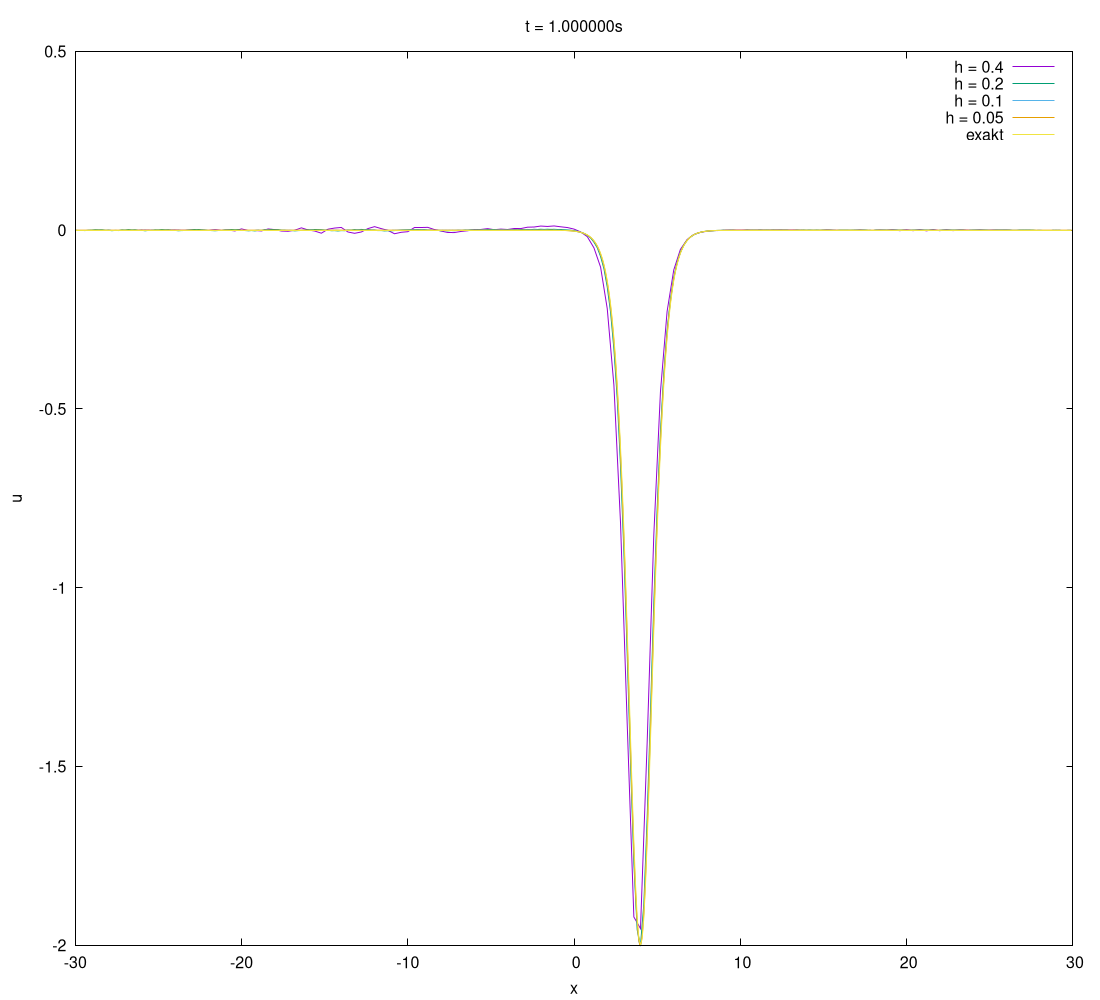
\includegraphics[width=0.48\textwidth]{vergleichN1.png}
	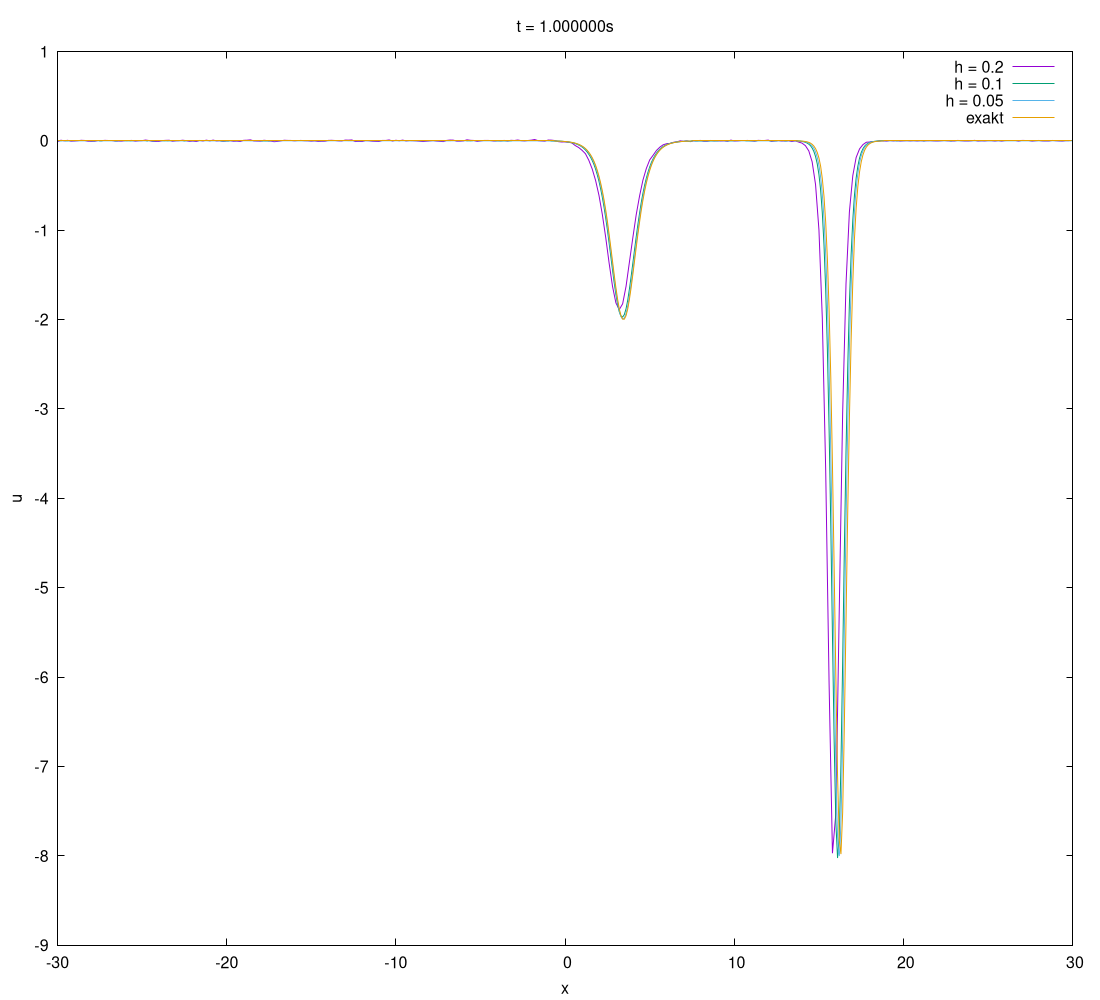
\includegraphics[width=0.48\textwidth]{vergleichN2.png}
	\caption[Vergleich]{Hier sind numerische und analytische Lösung der DGL für $N=1$ (links) und $N=2$ (rechts) mit $h=0.05, 0.1, 0.2, 0.4$ verglichen.}
	\label{fig:H10.22}
\end{figure}

Man kann sehr gut erkennen, dass die numerischen und analytischen Werte gut übereinstimmen, allerdings lassen sich die Abweichungen für großer Werte von $h$ erkennen. Einerseits dadurch, dass die Minima der Solitonen von der analytischen Lösung abweichen und daran, dass die Kurven nicht so glatt sind. Insgesamt, kann man das numerische Verfahren zur Lösung aber als sehr gut bewerten, da es für kleine $h$ sehr gute Werte ermittelt.


Um die Stabilität zu analysieren haben wir nun die numerischen Lösungen mit den jeweils gegebenen analytischen Lösungen für $N=1,2$ verglichen. Dafür haben wir für alle beliebigen Kombinationen von $0.05 \le h \le 0.4$ und $\le d \le$ genutzt um die Lösung numerisch zu bestimmen. Dann haben wir die Beträge der absoluten Abweichungen zwischen analytischem und numerischem Wert im Bereich $0 \le t \le 1$ berechnet und diese Abweichungen gemittelt. So hatten wir einen Abweichungswert für jede Kombination von $h$ und $d$. Dies haben wir dann für $N=1,2$ durchgeführt und jeweils in einer Heatmap dargestellt, siehe Abbildung \ref{fig:H10.2}.

\begin{figure}[htbp]
	\centering
	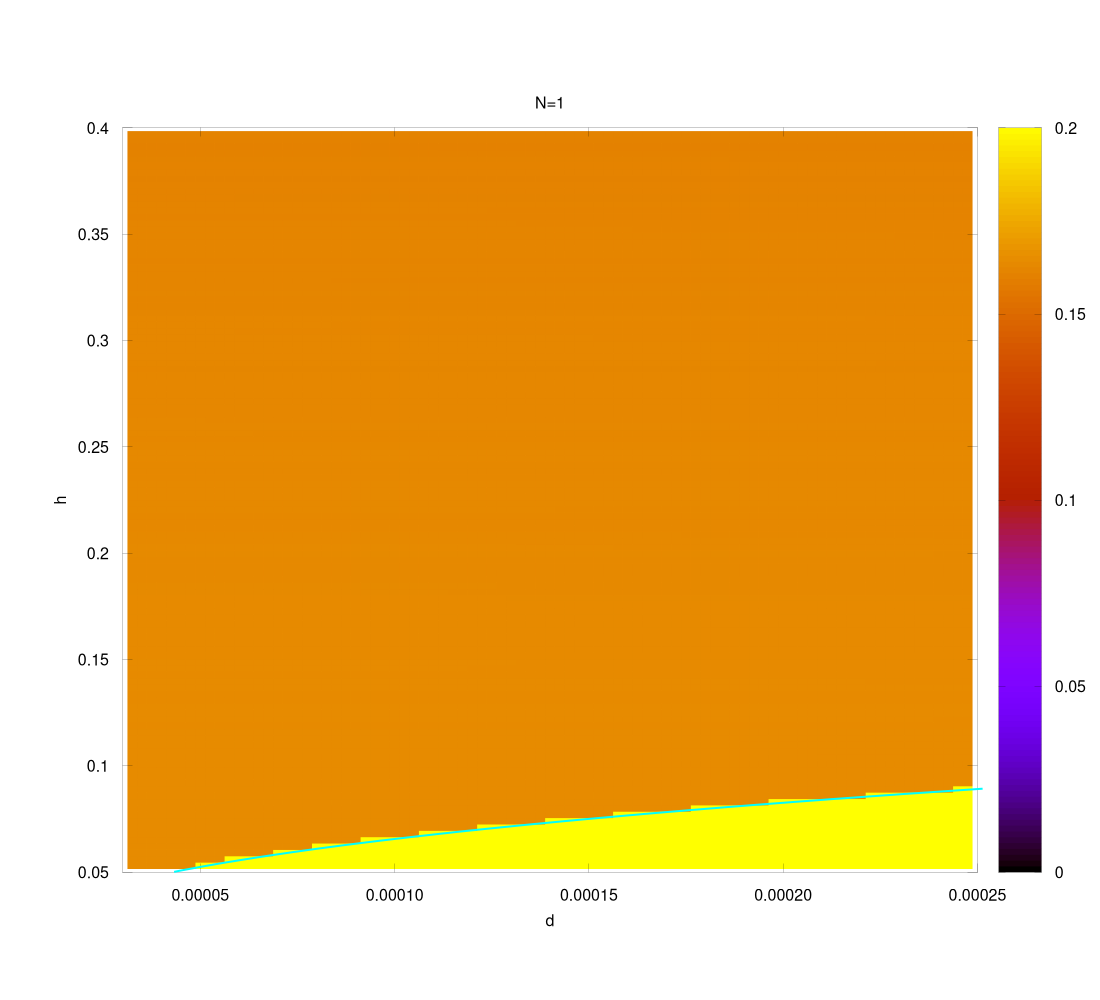
\includegraphics[width=0.48\textwidth]{heatMapN1}
	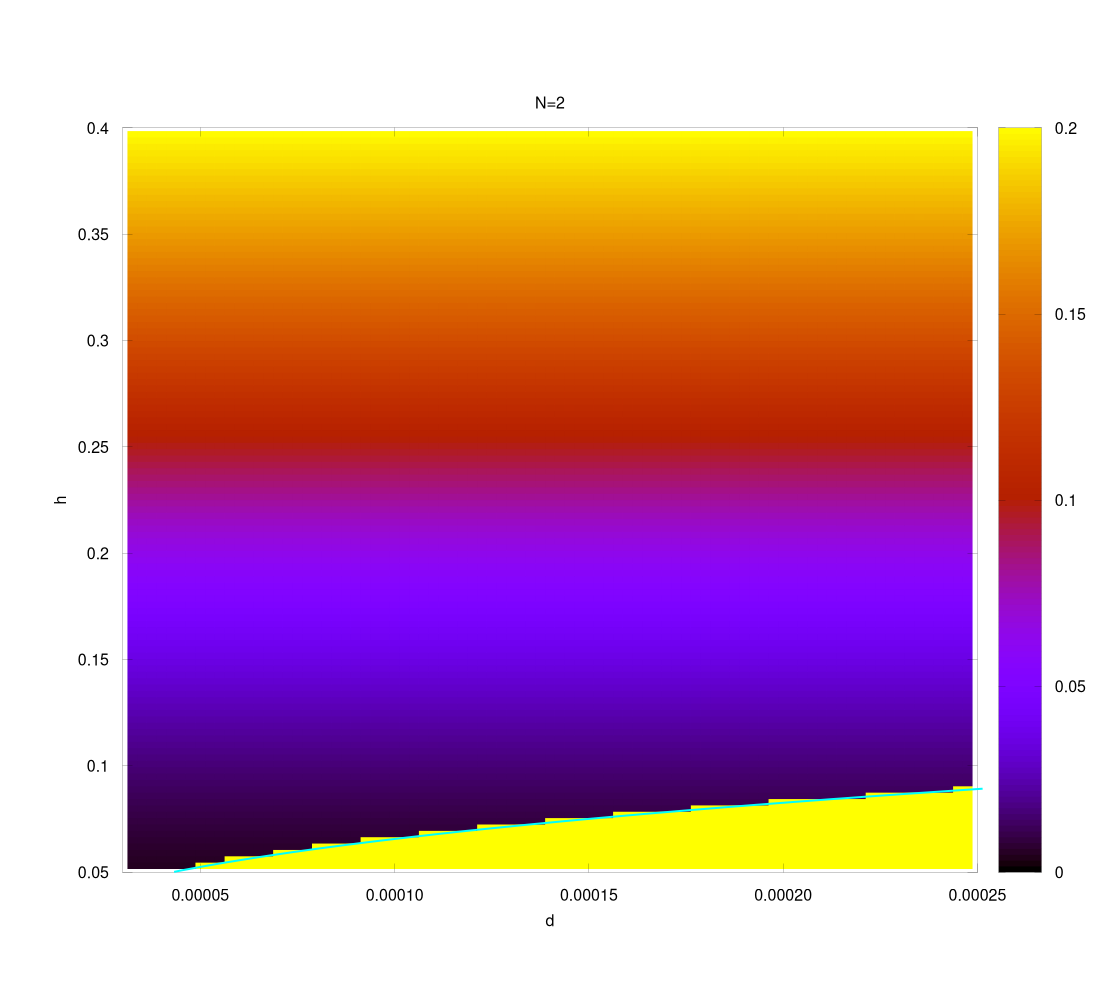
\includegraphics[width=0.48\textwidth]{heatMapN2}
	\caption[Vergleich]{Hier sind die Differenzen der numerischen und analytischen Lösung der DGL für $N=1$ (links) und $N=2$ (rechts) verglichen.}
	\label{fig:H10.2}
\end{figure}


In türkis ist in der Heatmap der Zusammenhang $ d= \frac{1}{2.6} \cdot h^3$ eingezeichnet. Es lässt sich sehr gut der Zusammenhang zwischen Größe der Fehler und dieser Kurve zeigen. Wir können also bestätigen, dass der gegebene Zusammenhang für stabil laufende Prozesse richtig ist.



\subsection{}

Nun haben wir $u^{[3]}(t, x)$ numerisch berechnet und anschließend in den Intervallen $ 0 \le t \le 1$ und $-5 \le x \le 45$ dargestellt. Dies haben wir wieder in Videoform umgesetzt, um den zeitlichen Verlauf adäquat darstellen zu können (siehe Video \ref{vid:H10.3}). 

\begin{figure}[htbp]
	\centering
	\includemedia[
	width=0.5525\linewidth,height=0.5\linewidth,
	activate=pageopen,
	transparent,
	addresource=N3.mp4,
	flashvars={
		source=N3.mp4     % same path as in addresource!
		&loop=true           % loop video
		&scaleMode=letterbox % preserve aspect ratio
	}
	]{}{VPlayer9.swf}
	\caption[]{Hier ist $u^{[3]}(t, x)$ im Bereich von $0\le t \le 1$ und $-5 \le x \le 45$ dargestellt.}
	\label{vid:H10.3}
\end{figure}

Es lassen sich hier wiederum sehr eindeutig die 3 Solitonen erkennen, die sich mit jeweils unterschiedlicher Geschwindigkeit bewegen und zum Zeitpunkt $t=0$ vollständig überlagern.




\subsection{}

Zuletzt haben wir noch die Lösungen für $1.1 \le N \le 1.9$ betrachtet und wie in den vorherigen Aufgaben den zeitlichen Verlauf von $u^{[N]}(x)$ als Video dargestellt. Um hier nicht neun einzelne Videos einbinden zu müssen, haben wir alle zeitlichen Entwicklungen in einem Diagramm (Video \ref{vid:H10.4}) dargestellt.

\begin{figure}[htbp]
	\centering
	\includemedia[
	width=0.5525\linewidth,height=0.5\linewidth,
	activate=pageopen,
	transparent,
	addresource=Nalle.mp4,
	flashvars={
		source=Nalle.mp4     % same path as in addresource!
		&loop=true           % loop video
		&scaleMode=letterbox % preserve aspect ratio
	}
	]{}{VPlayer9.swf}
	\caption[]{Hier ist $u^{[N]}(t, x)$ für $1.1 \le N \le 1.9$ dargestellt.}
	\label{vid:H10.4}
\end{figure}


Wie zu erwarten war, bilden sich, je näher der Wert $N$ an 2 ist, immer stärker 2 Solitonen aus. Zum Vergleich lässt sich auch der Wert für $N=1.0$ betrachten, der deutlich nur ein Soliton zeigt.



\end{document}


